\chapter{Results}\label{results}
\begin{comment}
In this chapter, we present the results of our investigation into the use of zero-cost proxies in neural architecture search (NAS) for graph convolutional networks (GCN). We address three research questions about using proxies in NAS for GCN, as outlined in the introduction chapter (\ref{section:goalsandrq}). Specifically, we analyze the effectiveness of different zero-cost proxies in ranking GCN architectures, examine the impact of incorporating proxies in the NAS algorithm and investigate the effectiveness of using an ensemble of proxies in NAS.
\end{comment}

\begin{comment}
Chapter 5 of the thesis presents the results of an investigation into the use of zero-cost proxies in neural architecture search for graph convolutional networks. The chapter includes a section on correlation and a vote section that analyze the effectiveness of different zero-cost proxies in ranking GCN architectures. Additionally, a section on supervised learning using Recursive Feature Elimination with Cross-Validation and Pointwise Ranking with Regression and Cross-Validation is included. Finally, the chapter addresses three research questions about the use of proxies in NAS for GCN and examines the impact of incorporating proxies in the NAS algorithm and investigates the effectiveness of using an ensemble of proxies in NAS.
\end{comment}

This chapter outlines the study's findings, responding to the defined research questions. Next, the 'Correlation Analysis' section evaluates the capability of zero-cost proxies in ranking GCN architectures concerning their validation accuracy. Subsequently, the analysis of correlation during the warm-up phase of GCN training is identified. Lastly, the 'Vote' and 'Weighted Arithmetic Mean' section examines techniques for combining zero-cost proxies to improve efficiency and accuracy in NAS algorithms.


\section{Correlation Analysis}\label{res:correlation}

The establishment of a benchmark provided the foundation for investigating the correlation between various zero-cost proxies and the ground truth represented by the validation accuracy. The Spearman Rank Correlation was employed to measure the correlation, as discussed in \cref{sec:corr}. 

\Cref{tab:corr} displays the obtained results, utilising the 693 architectures derived from the created benchmark. 
\clearpage

\begin{table}[h]
\caption{Correlation coefficients between proxy scores and model performance before training}
\centering
\begin{tabular}{lr}
\textbf{Name} & \textbf{$\rho$} \\ \hline
\multicolumn{1}{l|}{\cellcolor{verylightgray}epe\_nas} & \cellcolor{verylightgray}$0.0090$ \\
\multicolumn{1}{l|}{fisher} & $0.2405$ \\
\multicolumn{1}{l|}{\cellcolor{verylightgray}flops} & \cellcolor{verylightgray}$0.7241$ \\
\multicolumn{1}{l|}{grad\_norm} & $0.2653$ \\
\multicolumn{1}{l|}{\cellcolor{verylightgray}grad\_sign} & \cellcolor{verylightgray}$0.4979$ \\
\multicolumn{1}{l|}{grasp} & $-0.4244$ \\
\multicolumn{1}{l|}{\cellcolor{verylightgray}jacov} & \cellcolor{verylightgray}$-0.0465$ \\
\multicolumn{1}{l|}{l2\_norm} & $0.7325$ \\
\multicolumn{1}{l|}{\cellcolor{verylightgray}nwot} & \cellcolor{verylightgray}$0.1214$ \\
\multicolumn{1}{l|}{params} & $0.6164$ \\
\multicolumn{1}{l|}{\cellcolor{verylightgray}plain} & \cellcolor{verylightgray}$0.2490$ \\
\multicolumn{1}{l|}{snip} & $0.2468$ \\
\multicolumn{1}{l|}{\cellcolor{verylightgray}synflow} & \cellcolor{verylightgray}0.7599 \\
\multicolumn{1}{l|}{zen} & \textbf{0.7827} \\
\end{tabular}
\label{tab:corr}
\end{table}

\begin{comment}
\begin{figure}[h!]
  \centering
  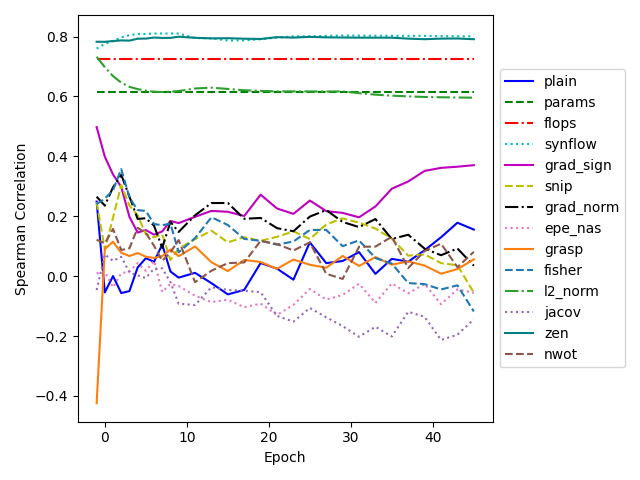
\includegraphics[width=0.8\columnwidth]{figures/correlations.png}
  \caption{Correlations for all zero-cost proxies over multiple epochs}
  \label{fig:warmup}
\end{figure}
\end{comment}


The results in \cref{tab:corr} reveal that specific proxies correlate strongly with the validation accuracy, while others demonstrate weaker correlations. \Cref{tab:corr} indices that Zen has the highest correlation with model performance, with a coefficient of $0.7827$. Synflow is also performing well, with a coefficient of $0.7599$. This suggests that both Zen and synflow are the most effective zero-cost proxies among the ones considered in this study. 

Conversely, the epe\_nas and jacov proxies exhibit a weak correlation with the model performance, with coefficients of $0.0090$ and $-0.0465$, respectively. 

It is also worth noting that the l2\_norm, flops, and params proxies show relatively strong correlations with coefficients of $0.7325$, $0.7241$, and $0.6164$, respectively. Although these proxies might be less effective than Zen and synflow, they still demonstrate considerable potential for predicting model performance.

The findings of this correlation analysis provide valuable insights into the predictive capacity of each proxy in relation to the ground truth. This understanding can inform the development of more efficient and effective NAS approaches, thereby reducing computational demands and enabling more rapid progress in the field.

\subsection{Vote}

After sorting, the results will only display the top-5 combinations as too many values will be shown. However, from the results shown in \cref{tab:vote}, all combinations of metrics exhibit almost the same custom correlation measure (majority vote score) of $ > 0.788$. This suggests that these combinations of metrics perform similarly in terms of the agreement between the majority of metrics and accuracy differences.

\begin{table}[h!]
\caption{Vote scores}
\centering
\begin{tabular}{ll}
\textbf{Name} & \textbf{Value} \\ \hline
\multicolumn{1}{l|}{synflow, zen, fisher} & \textbf{0.7899} \\
\multicolumn{1}{l|}{\cellcolor{verylightgray}synflow, zen, nwot} & \cellcolor{verylightgray}$0.7888$ \\
\multicolumn{1}{l|}{synflow, zen, flops} & $0.7885$ \\
\multicolumn{1}{l|}{\cellcolor{verylightgray}synflow, zen, plain} & \cellcolor{verylightgray}$0.7883$ \\
\multicolumn{1}{l|}{synflow, zen, grad\_norm} & $0.7883$ \\
\end{tabular}
\label{tab:vote}
\end{table}

It is important to note that these results are based on the custom correlation measure (see \cref{subsec:vote}), which differs from standard correlation measures such as Spearman's rank correlation. The custom correlation measure captures the extent to which the majority of metric differences agree with the differences in dataset accuracies. A higher correlation value indicates a stronger agreement, while a lower correlation value suggests a weaker agreement.

\subsection{Warmup}


\Cref{fig:warmup,fig:warmup_seperate} present the variation in correlation during the initial ten epochs, with epoch -1 representing the starting correlations (same as \cref{tab:corr}). The figure demonstrates that \gls{SynFlow} and Zen exhibit the highest performance, maintaining a stable correlation at $\approx 0.8$ throughout the observed epochs. A minor increment in correlation can be observed, although its impact is relatively insignificant. Furthermore, params, l2\_norm, and \gls{FLOPs} exhibit consistently strong performance with a correlation coefficient ($\rho$) exceeding $0.6$ across all epochs under consideration.

\begin{figure}[!ht]
  \centering
  \includesvg[width=0.8\columnwidth]{figures/correlations.svg}
  \caption{Correlations for all zero-cost proxies over multiple epochs}
  \label{fig:warmup}
\end{figure}

\clearpage

\begin{figure}[htbp]
  \centering
    \begin{adjustbox}{width=1.2\columnwidth,center}
  \begin{tabular}{ccc}
    \includesvg[width=0.5\textwidth]{figures/correlations/epe_nas_correlations.svg} &
    \includesvg[width=0.5\textwidth]{figures/correlations/fisher_correlations.svg} &
    \includesvg[width=0.5\textwidth]{figures/correlations/flops_correlations.svg} \\
    \includesvg[width=0.5\textwidth]{figures/correlations/grad_norm_correlations.svg} &
    \includesvg[width=0.5\textwidth]{figures/correlations/grad_sign_correlations.svg} &
    \includesvg[width=0.5\textwidth]{figures/correlations/grasp_correlations.svg} \\
    \includesvg[width=0.5\textwidth]{figures/correlations/jacov_correlations.svg} &
    \includesvg[width=0.5\textwidth]{figures/correlations/l2_norm_correlations.svg} &
    \includesvg[width=0.5\textwidth]{figures/correlations/nwot_correlations.svg} \\
    \includesvg[width=0.5\textwidth]{figures/correlations/params_correlations.svg} &
    \includesvg[width=0.5\textwidth]{figures/correlations/plain_correlations.svg} &
    \includesvg[width=0.5\textwidth]{figures/correlations/snip_correlations.svg} \\
    \includesvg[width=0.5\textwidth]{figures/correlations/\gls{synflow}_correlations.svg} &
    \includesvg[width=0.5\textwidth]{figures/correlations/zen_correlations.svg} 
  \end{tabular}
  \end{adjustbox}
  \caption{Each zero-cost proxy with the correlation over multiple epochs}
  \label{fig:warmup_seperate}
\end{figure}

\section{Weighted Arithmetic Mean}

\Cref{fig:weighted} displays a scatter plot illustrating the relationship between validation accuracy and the weighted arithmetic mean. Every data point displayed within the graph corresponds to a unique architecture evaluated during the experiment. A dotted red line represents the best-fit linear regression line through the data points. Additionally, the graph includes Spearman's rank correlation coefficient in the title, which measures the monotonic relationship between the validation accuracy and the weighted arithmetic mean. 

\begin{figure}[h!]
  \centering
  \includesvg[width=0.9\columnwidth]{figures/weighted_average.svg}
  \caption{Weighted Arithmetic Mean}
  \label{fig:weighted}
\end{figure}



%
\section{Supervised Learning}
\subsection{Recursive Feature Elimination with Cross-Validation}
This section presents the feature selection results using Recursive Feature Elimination with Cross-Validation (RFECV) and its impact on the model's performance. Our initial dataset consists of 14 zero-cost proxy features, and our goal is to identify the optimal subset of features that would lead to the highest R2 score in our regression model.

We employed the RFECV algorithm for feature selection, which iteratively eliminates the least essential features from the dataset based on their importance, as determined by the model's coefficients or feature importances. The model performance is evaluated using cross-validation at each iteration, and the optimal number of features is chosen based on the highest R2 score.

Upon applying the RFECV algorithm, only one feature was selected as optimal, implying that this single feature provides the highest R2 score during cross-validation. However, the resulting R2 score on the test set is 0.14, indicating that the selected feature explains only a tiny portion of the variance in the target variable.

\subsection{Pointwise Ranking with Regression and Cross-Validation}

\kommentar{Hvor er det mentioned??}{}

As mentioned in \cref{}, one approach used supervised learning with pointwise ranking and cross-validation to assess the performance of combining zero-cost proxies. Our analysis involved training a linear regression model to predict the performance of various \gls{GCN} architectures based on the combined zero-cost proxy features. We then ranked the architectures based on their predicted performance scores and evaluated the ranking quality using measures such as Mean Squared Error (MSE) and Normalized Discounted Cumulative Gain (NDCG). The results are presented for the approach without cross-validation and the refined approach with cross-validation.

\begin{table}[h]
\centering
\begin{tabular}{ll}
\textbf{Evaluation Method}             & \textbf{Mean Squared Error} \\ \hline
\multicolumn{1}{l|}{Without Cross-Validation} & 0.00108281          \\
\multicolumn{1}{l|}{\cellcolor{verylightgray}With Cross-Validation} & \cellcolor{verylightgray}0.00145585 \\ \hline
\end{tabular}
\begin{tabular}{ll}
\textbf{Evaluation Method}             & \textbf{NDCG} \\ \hline
\multicolumn{1}{l|}{Without Cross-Validation} & 0.9999999999999997          \\
\multicolumn{1}{l|}{\cellcolor{verylightgray}With Cross-Validation} & \cellcolor{verylightgray}0.9999999999999997 \\ \hline
\end{tabular}
\caption{Comparison of pointwise ranking results with and without cross-validation}
\label{tab:ranking_results}
\end{table}


\Cref{tab:ranking_results} summarizes the results of our experiments. The Mean Squared Error (MSE) and Normalized Discounted Cumulative Gain (NDCG) scores are reported for both the original approach without cross-validation and the approach with cross-validation.

Without cross-validation, the model achieved an MSE of 0.00108281 and an NDCG score of 0.9999999999999997. When using cross-validation, the model achieved an MSE of 0.00145585 and an NDCG score of 0.9999999999999997 (averaged over cross-validation folds).



